\chapter{Package and Pinout}
\label{ch:package-and-pinout}

\section{Chip Layout}

The SIRC-1 is provided in a 64-pin dual in-line package (DIP-64).

\begin{figure}[htbp]
	\centering
	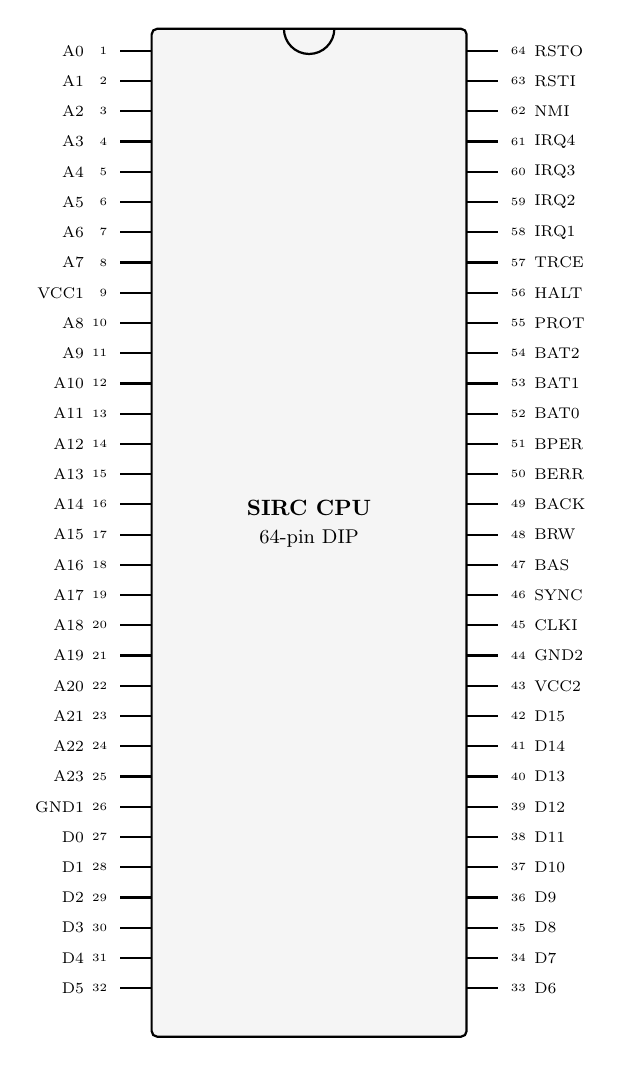
\begin{tikzpicture}[
			scale=0.8,
			transform shape,
			pinlabel/.style={font=\scriptsize},
			pinnum/.style={font=\tiny},
			body/.style={draw, thick, rounded corners=2pt, fill=gray!8},
			pin/.style={draw, thick}
		]

		% Package body
		\draw[body] (0,0) rectangle (5,-16);

		% Notch
		\draw[thick] (2.1,0) arc[start angle=180,end angle=360,radius=0.4];

		% Left-side pins: 1-32, top to bottom
		\foreach \n/\name in {
				1/A0,
				2/A1,
				3/A2,
				4/A3,
				5/A4,
				6/A5,
				7/A6,
				8/A7,
				9/VCC1,
				10/A8,
				11/A9,
				12/A10,
				13/A11,
				14/A12,
				15/A13,
				16/A14,
				17/A15,
				18/A16,
				19/A17,
				20/A18,
				21/A19,
				22/A20,
				23/A21,
				24/A22,
				25/A23,
				26/GND1,
				27/D0,
				28/D1,
				29/D2,
				30/D3,
				31/D4,
				32/D5
			} {
				\pgfmathsetmacro{\y}{-0.35 - (\n-1)*0.48}
				\draw[pin] (-0.5,\y) -- (0,\y);
				\node[pinnum, anchor=east] at (-0.58,\y) {\n};
				\node[pinlabel, anchor=east] at (-0.95,\y) {\name};
			}

		% Right-side pins: 64-33, top to bottom
		\foreach \n/\name [count=\i from 0] in {
				64/\activelow{RSTO},
				63/\activelow{RSTI},
				62/\activelow{NMI},
				61/\activelow{IRQ4},
				60/\activelow{IRQ3},
				59/\activelow{IRQ2},
				58/\activelow{IRQ1},
				57/\activelow{TRCE},
				56/\activelow{HALT},
				55/PROT,
				54/BAT2,
				53/BAT1,
				52/BAT0,
				51/\activelow{BPER},
				50/\activelow{BERR},
				49/\activelow{BACK},
				48/BRW,
				47/\activelow{BAS},
				46/SYNC,
				45/CLKI,
				44/GND2,
				43/VCC2,
				42/D15,
				41/D14,
				40/D13,
				39/D12,
				38/D11,
				37/D10,
				36/D9,
				35/D8,
				34/D7,
				33/D6
			} {
				\pgfmathsetmacro{\y}{-0.35 - \i*0.48}
				\draw[pin] (5,\y) -- (5.5,\y);
				\node[pinnum, anchor=west] at (5.58,\y) {\n};
				\node[pinlabel, anchor=west] at (5.95,\y) {\name};
			}

		% Package label
		\node[font=\bfseries] at (2.5,-7.6) {SIRC CPU};
		\node[font=\small] at (2.5,-8.1) {64-pin DIP};

	\end{tikzpicture}
	\caption{SIRC CPU 64-pin DIP Pinout, Top View}
\end{figure}

\begin{table}[H]
	\centering
	\begin{tabular}{rll}
		\toprule
		\textbf{Pin} & \textbf{Name}                      & \textbf{Description}           \\
		\midrule
		1--8         & A0--A7                             & Address bus bits 0--7          \\
		9            & VCC1                               & Power supply                   \\
		10--25       & A8--A23                            & Address bus bits 8--23         \\
		26           & GND1                               & Ground                         \\
		27--42       & D0--D15                            & Data bus bits 0--15            \\
		43           & VCC2                               & Power supply                   \\
		44           & GND2                               & Ground                         \\
		45           & CLKI                               & Clock input                    \\
		46           & SYNC                               & Instruction-sync output        \\
		47           & \activelow{BAS}                    & Bus access strobe output       \\
		48           & BRW                                & Bus read/write output          \\
		49           & \activelow{BACK}                   & Bus acknowledge input          \\
		50           & \activelow{BERR}                   & Bus error input                \\
		51           & \activelow{BPER}                   & Bus protection error input     \\
		52--54       & BAT0--BAT2                         & Bus access type bits 0--2      \\
		55           & PROT                               & Protected-mode output          \\
		56           & \activelow{HALT}                   & External CPU halt input        \\
		57           & \activelow{TRCE}                   & Force trace mode input         \\
		58--61       & \activelow{IRQ1}--\activelow{IRQ4} & Maskable interrupt inputs 1--4 \\
		62           & \activelow{NMI}                    & Non-maskable interrupt input   \\
		63           & \activelow{RSTI}                   & Reset input                    \\
		64           & \activelow{RSTO}                   & Reset output                   \\
		\bottomrule
	\end{tabular}
	\caption{SIRC CPU 64-pin DIP Pinout}
\end{table}
